\section{Introduction}

% Slide 1
\begin{frame}{What Happens When a Program Runs?}
  \begin{itemize}
    \item A running program executes instructions.
    \item The processor repeatedly \textbf{fetches}, \textbf{decodes}, and \textbf{executes} instructions.
    \item Programs assume an orderly, sequential execution model.
    \item The operating system works underneath this simple model to make the machine easier to use.
  \end{itemize}

  \vspace{0.5em}
  \begin{block}{Key idea}
    The OS hides much of the complexity involved in sharing and managing hardware resources.
  \end{block}
\end{frame}

% Slide 2
\begin{frame}{What Does an Operating System Do?}
  \begin{itemize}
    \item Makes it easier to run programs and use hardware resources.
    \item \textbf{Virtualizes} physical resources such as the CPU, memory, and storage.
    \item Provides interfaces through \textbf{system calls}.
    \item Acts as a \textbf{resource manager} for shared system resources.
  \end{itemize}

  \vspace{0.5em}
  \begin{alertblock}{The Crux of the Problem}
    How does the operating system virtualize resources efficiently, and what hardware support is needed?
  \end{alertblock}

  % Source location: shaded ``Crux of the Problem'' box, chapter page 2.
\end{frame}

% Slide 3
\begin{frame}{Virtualizing the CPU}
  \begin{columns}[T,onlytextwidth]
    \column{0.48\textwidth}
      \begin{itemize}
        \item The example program repeatedly waits and prints a user-provided string.
        \item A single program running alone is straightforward.
        \item The interesting behavior appears when several copies execute at once.
      \end{itemize}

    \column{0.50\textwidth}
    \begin{figure}
        \centering
        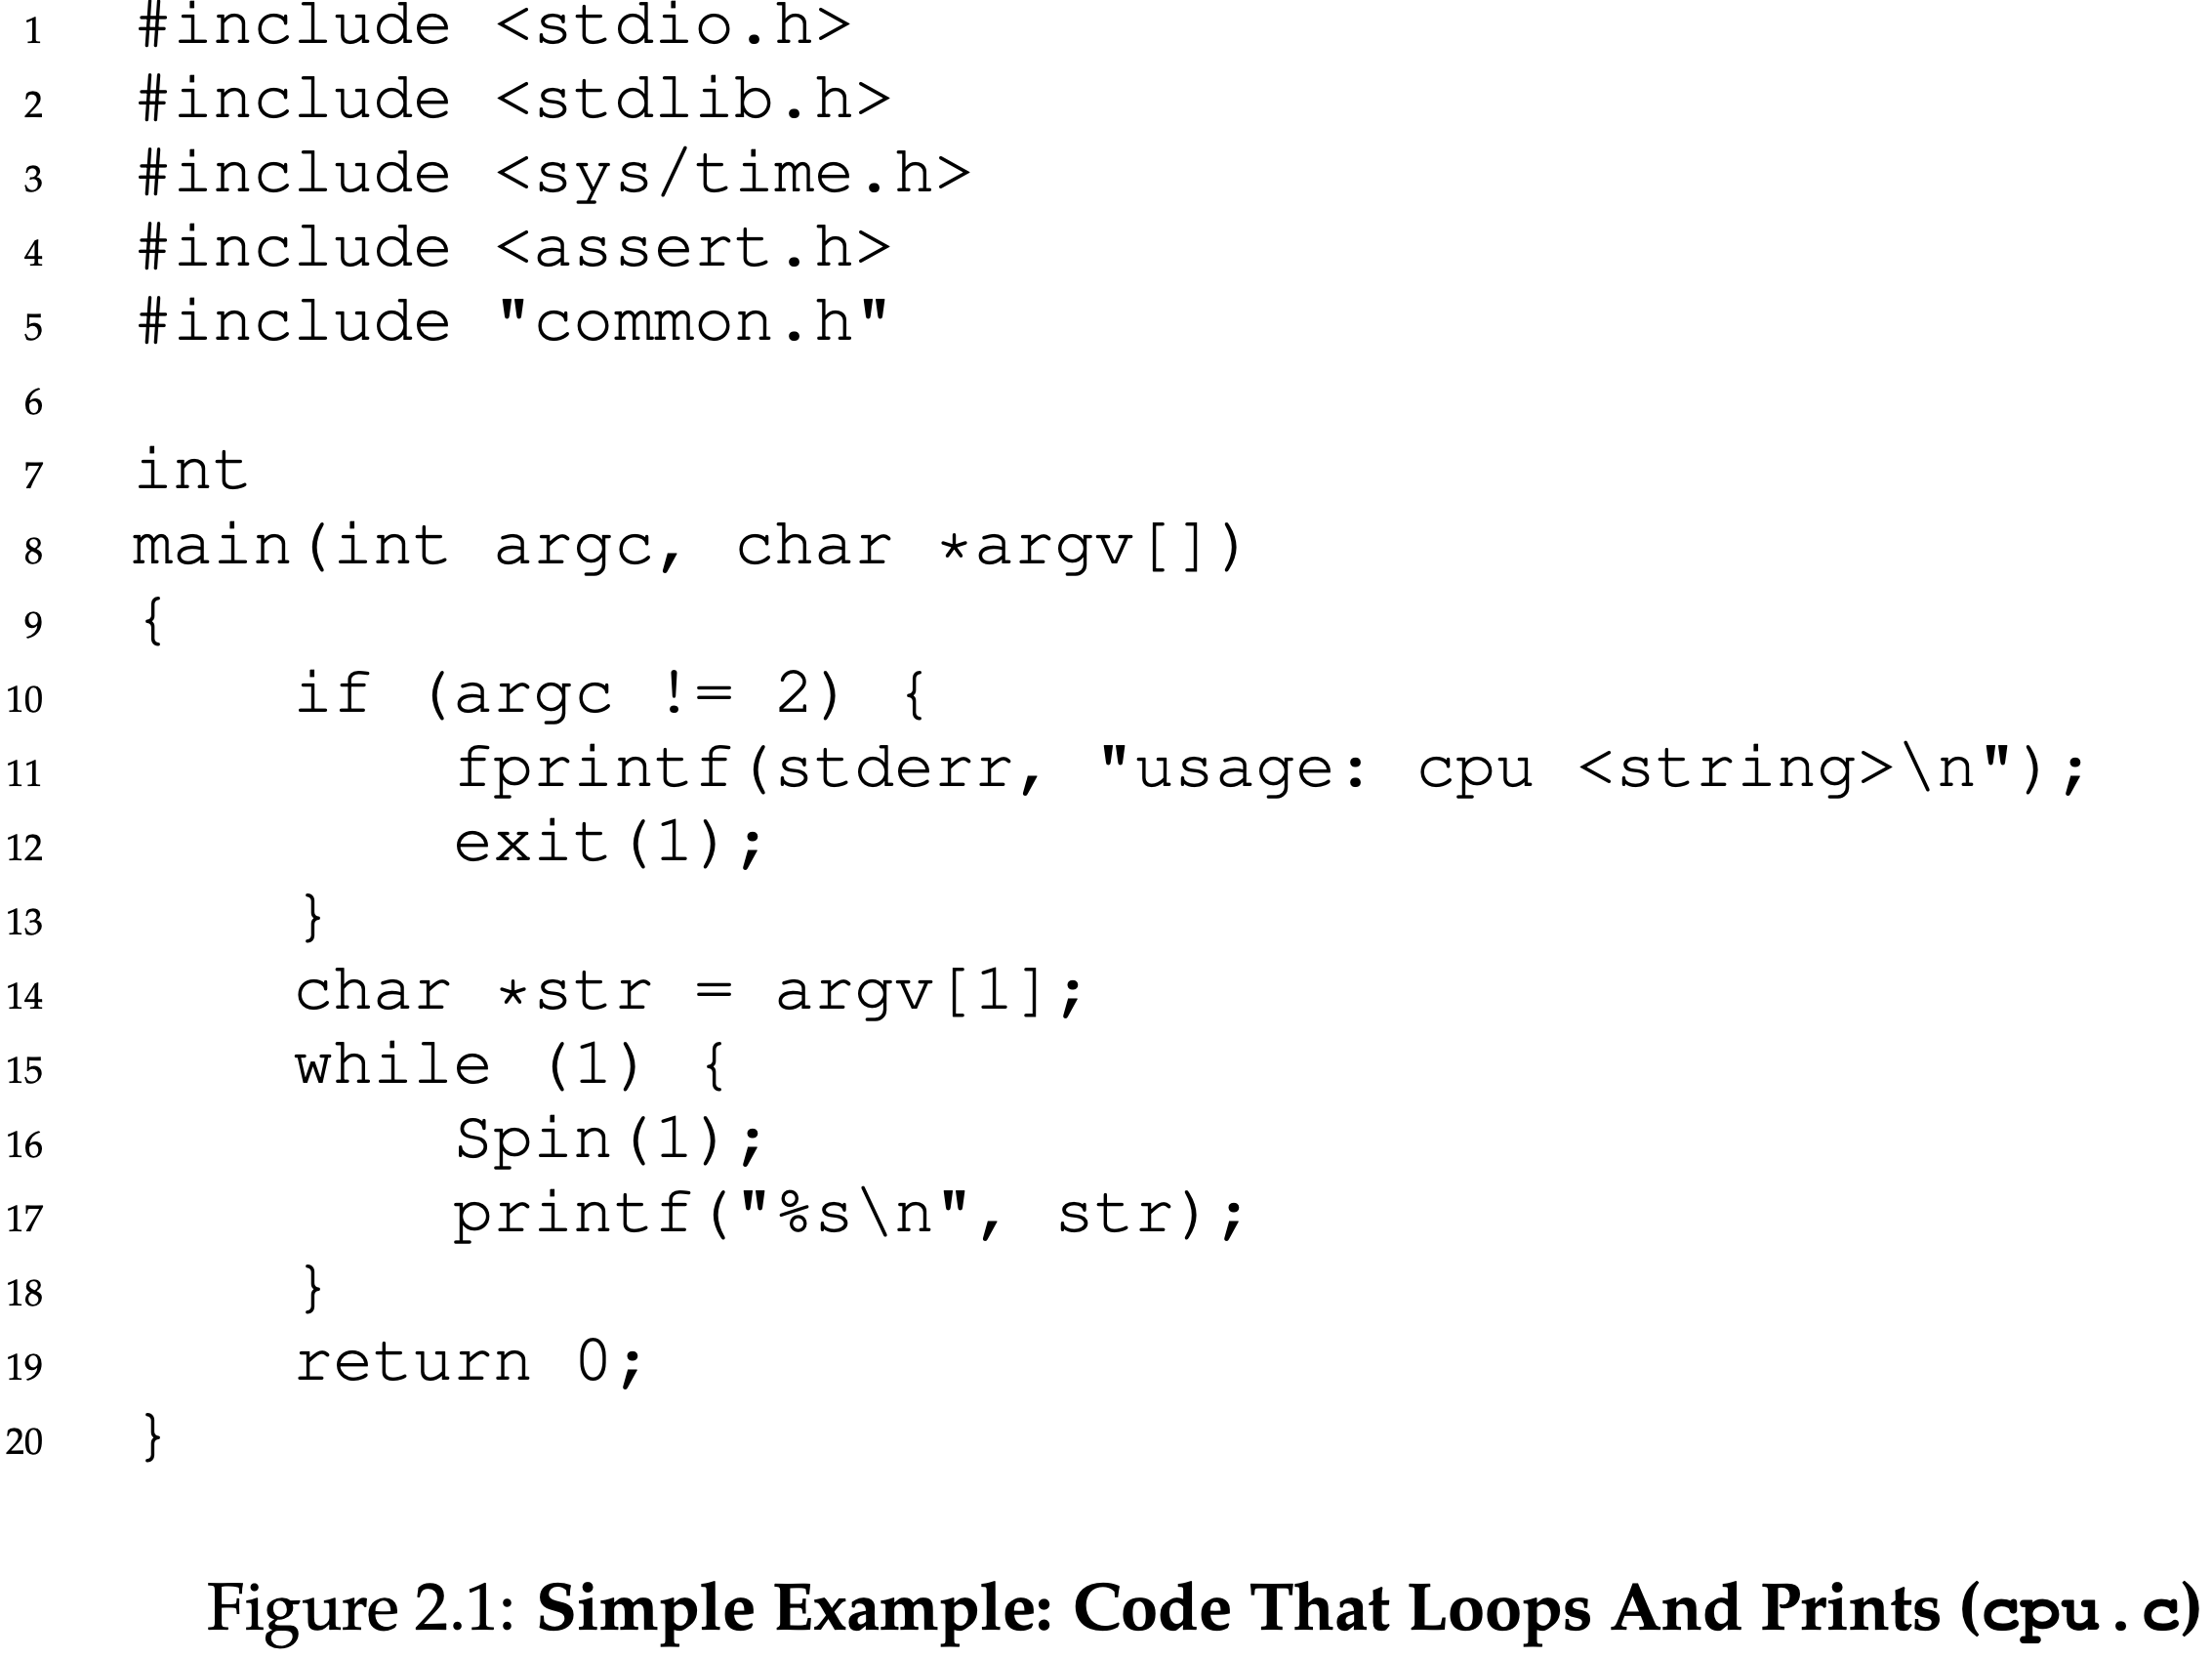
\includegraphics[width=1.1\linewidth]{figs/chapter-2/figure-2.1.png}
        \caption*{Source: chapter page 3.}
        \label{fig:figure-2.1}
    \end{figure}
      % \figureplaceholder{Figure 2.1: cpu.c}{Place the book figure here. Source: chapter page 3.}
  \end{columns}
\end{frame}

% Slide 4
\begin{frame}{The Illusion of Many CPUs}
  \begin{columns}[T,onlytextwidth]
    \column{0.48\textwidth}
    \begin{figure}
        \centering
        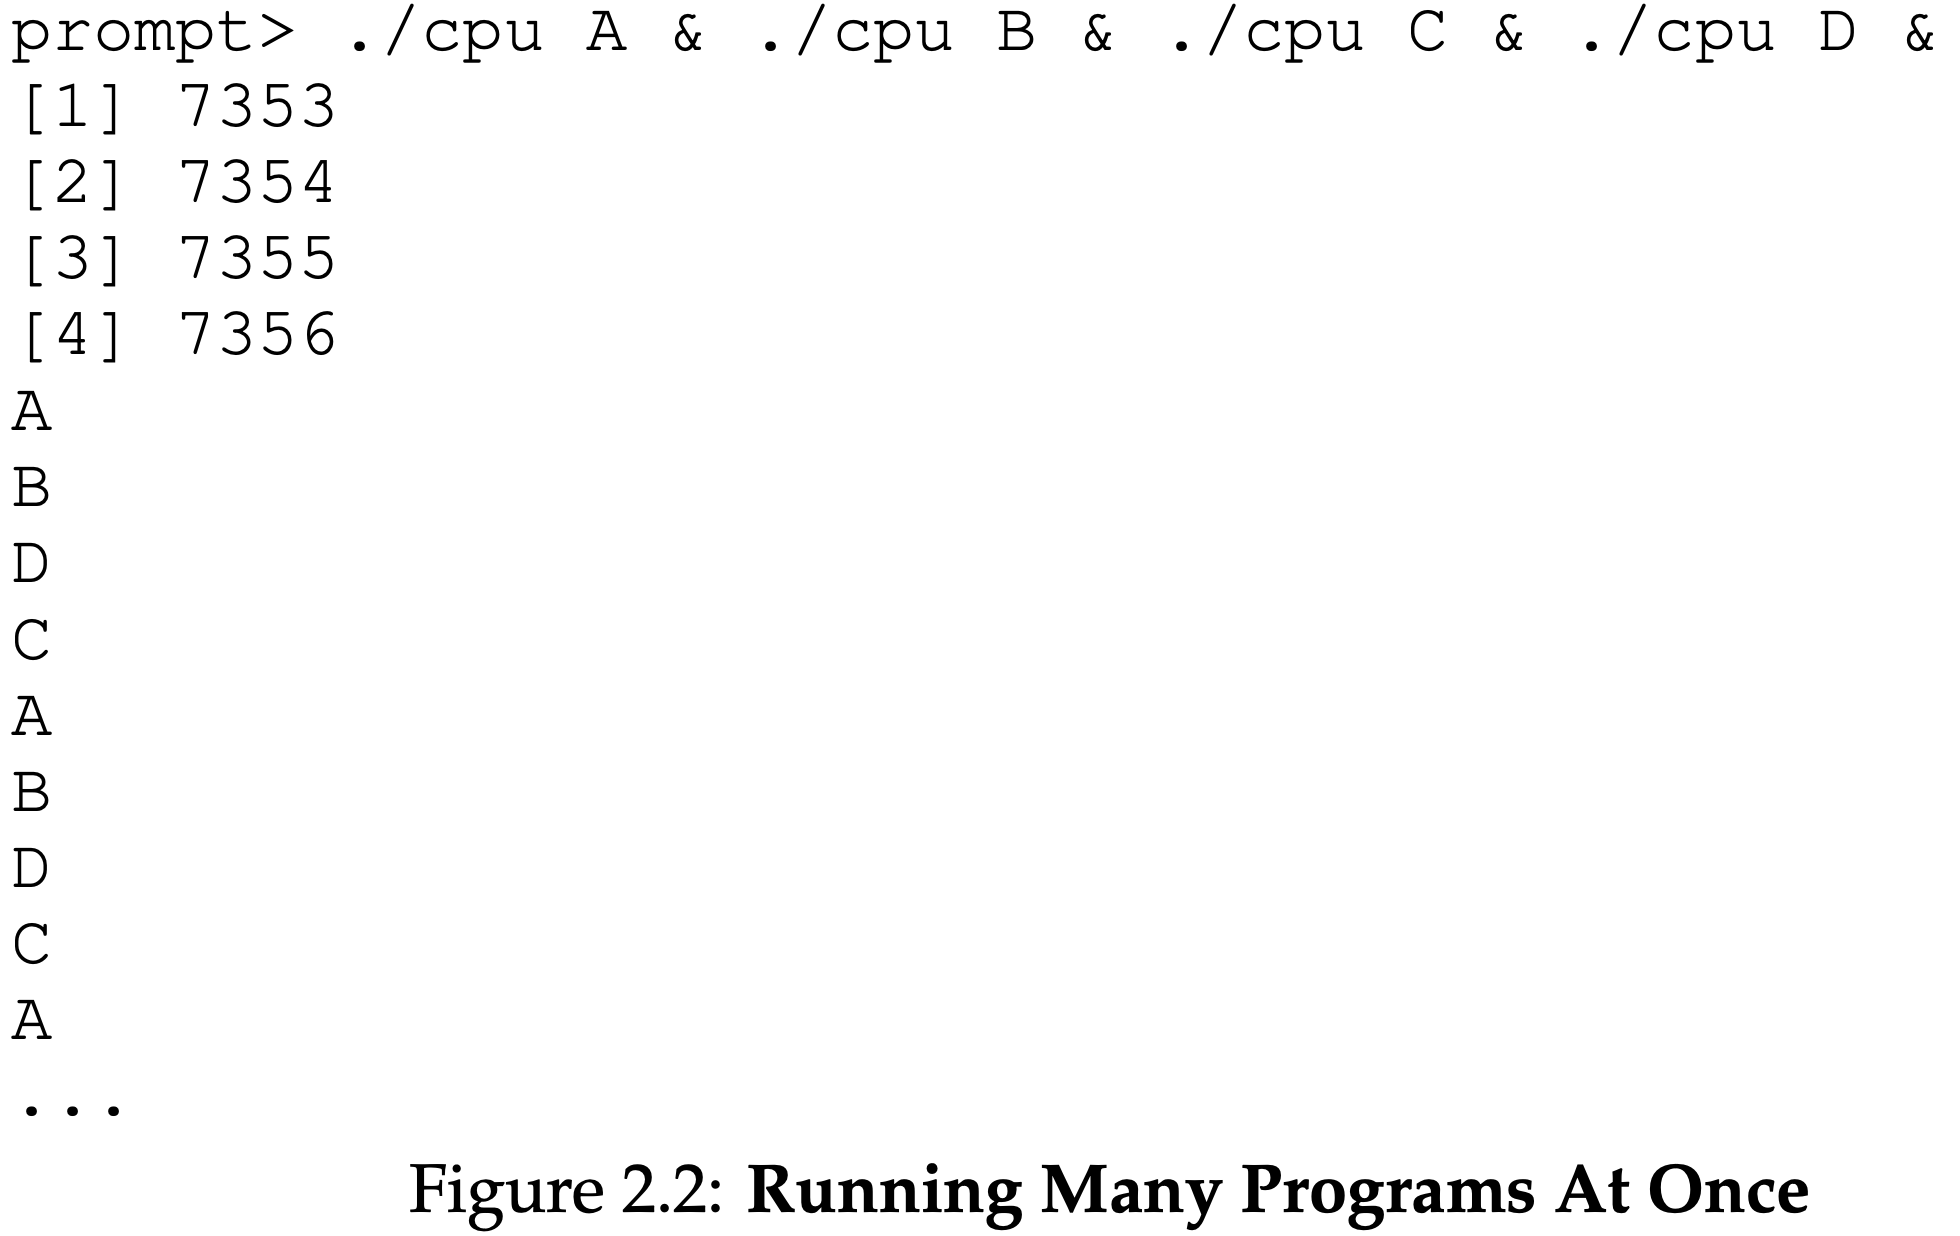
\includegraphics[width=1.1\linewidth]{figs/chapter-2/figure-2.2.png}
        \caption*{Source: chapter page 4.}
        \label{fig:figure-2.2}
    \end{figure}
      % \figureplaceholder{Figure 2.2: Running Many Programs At Once}{Place the book figure here. Source: chapter page 4.}

    \column{0.50\textwidth}
      \begin{itemize}
        \item Multiple programs appear to run simultaneously even on one processor.
        \item The OS, with hardware support, creates the illusion of many \textbf{virtual CPUs}.
        \item The OS also needs policies to decide which program should run at a given time.
      \end{itemize}
  \end{columns}
\end{frame}

% Slide 5
\begin{frame}{Virtualizing Memory}
  \begin{columns}[T,onlytextwidth]
    \column{0.48\textwidth}
      \begin{itemize}
        \item Memory can be viewed as an array of bytes addressed by the processor.
        \item Programs continuously access memory for instructions and data.
        \item The example allocates memory with \texttt{malloc()}, initializes it, and repeatedly updates it.
      \end{itemize}

    \column{0.50\textwidth}
    \begin{figure}
        \centering
        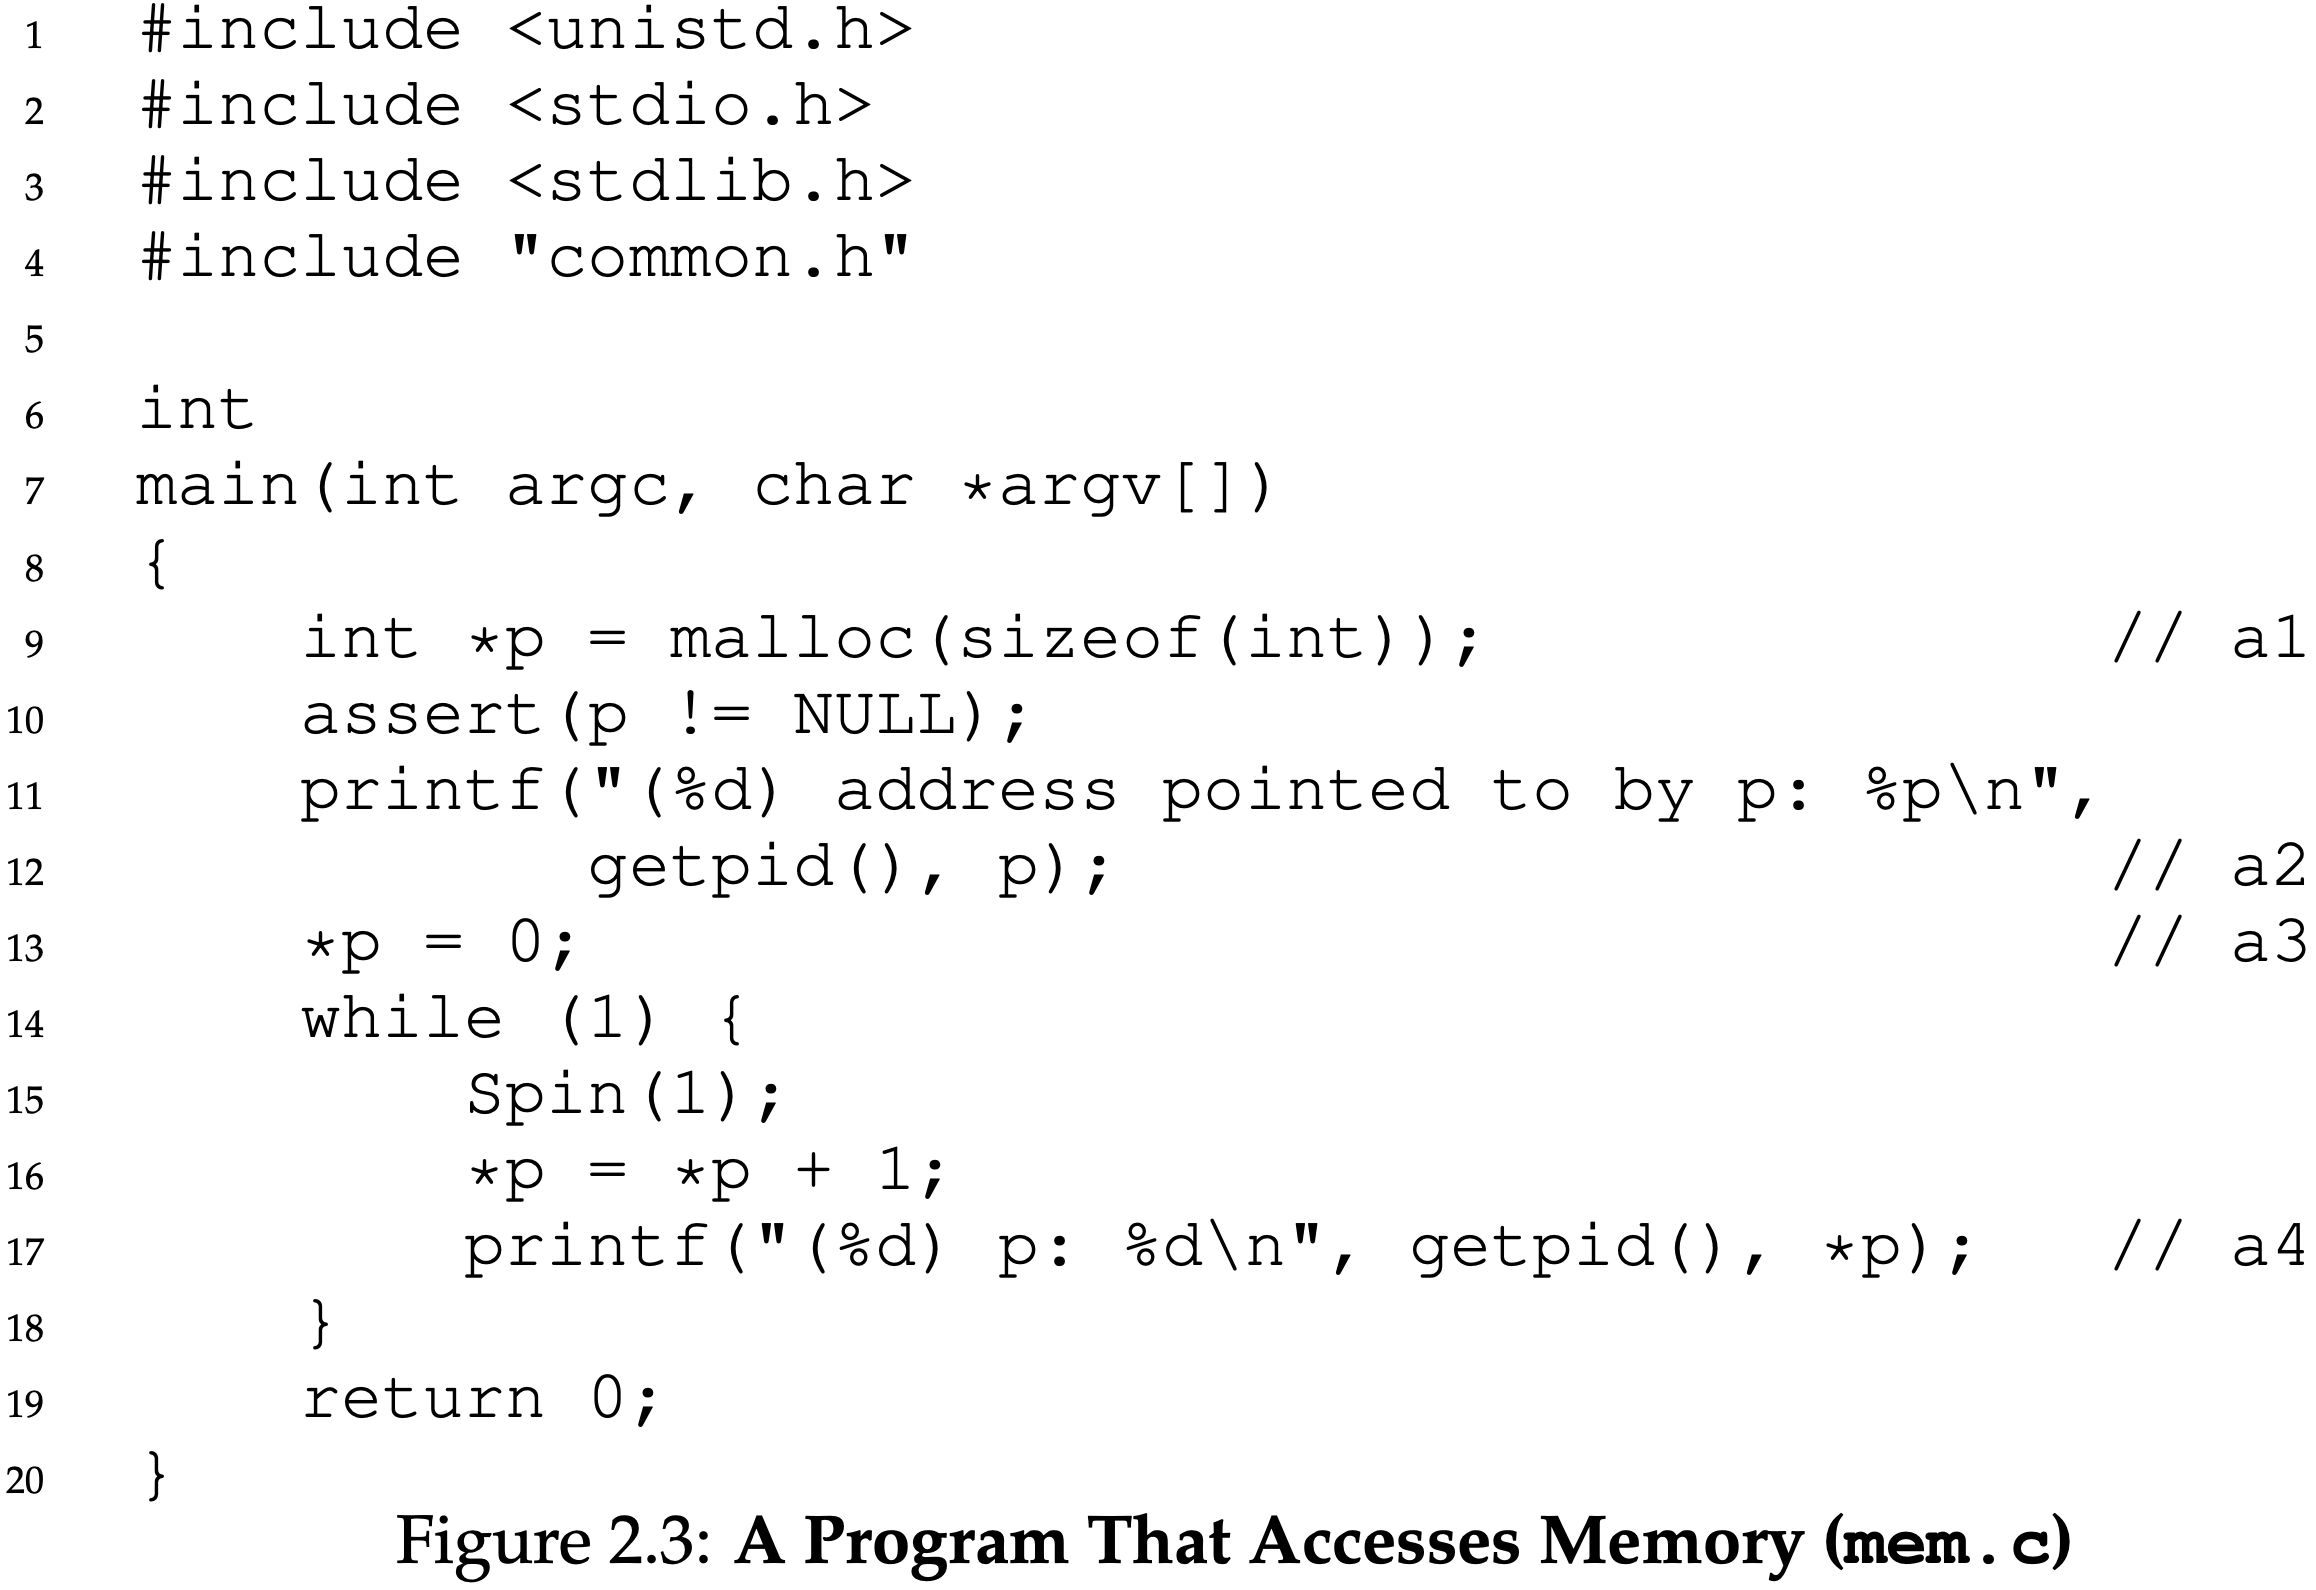
\includegraphics[width=1.1\linewidth]{figs/chapter-2/figure-2.3.png}
        \caption*{Source: chapter page 5.}
        \label{fig:figure-2.3}
    \end{figure}
      % \figureplaceholder{Figure 2.3: mem.c}{Place the book figure here. Source: chapter page 5.}
  \end{columns}
\end{frame}

% Slide 6
\begin{frame}{Private Virtual Address Spaces}
  \begin{columns}[T,onlytextwidth]
    \column{0.48\textwidth}
    \begin{figure}
        \centering
        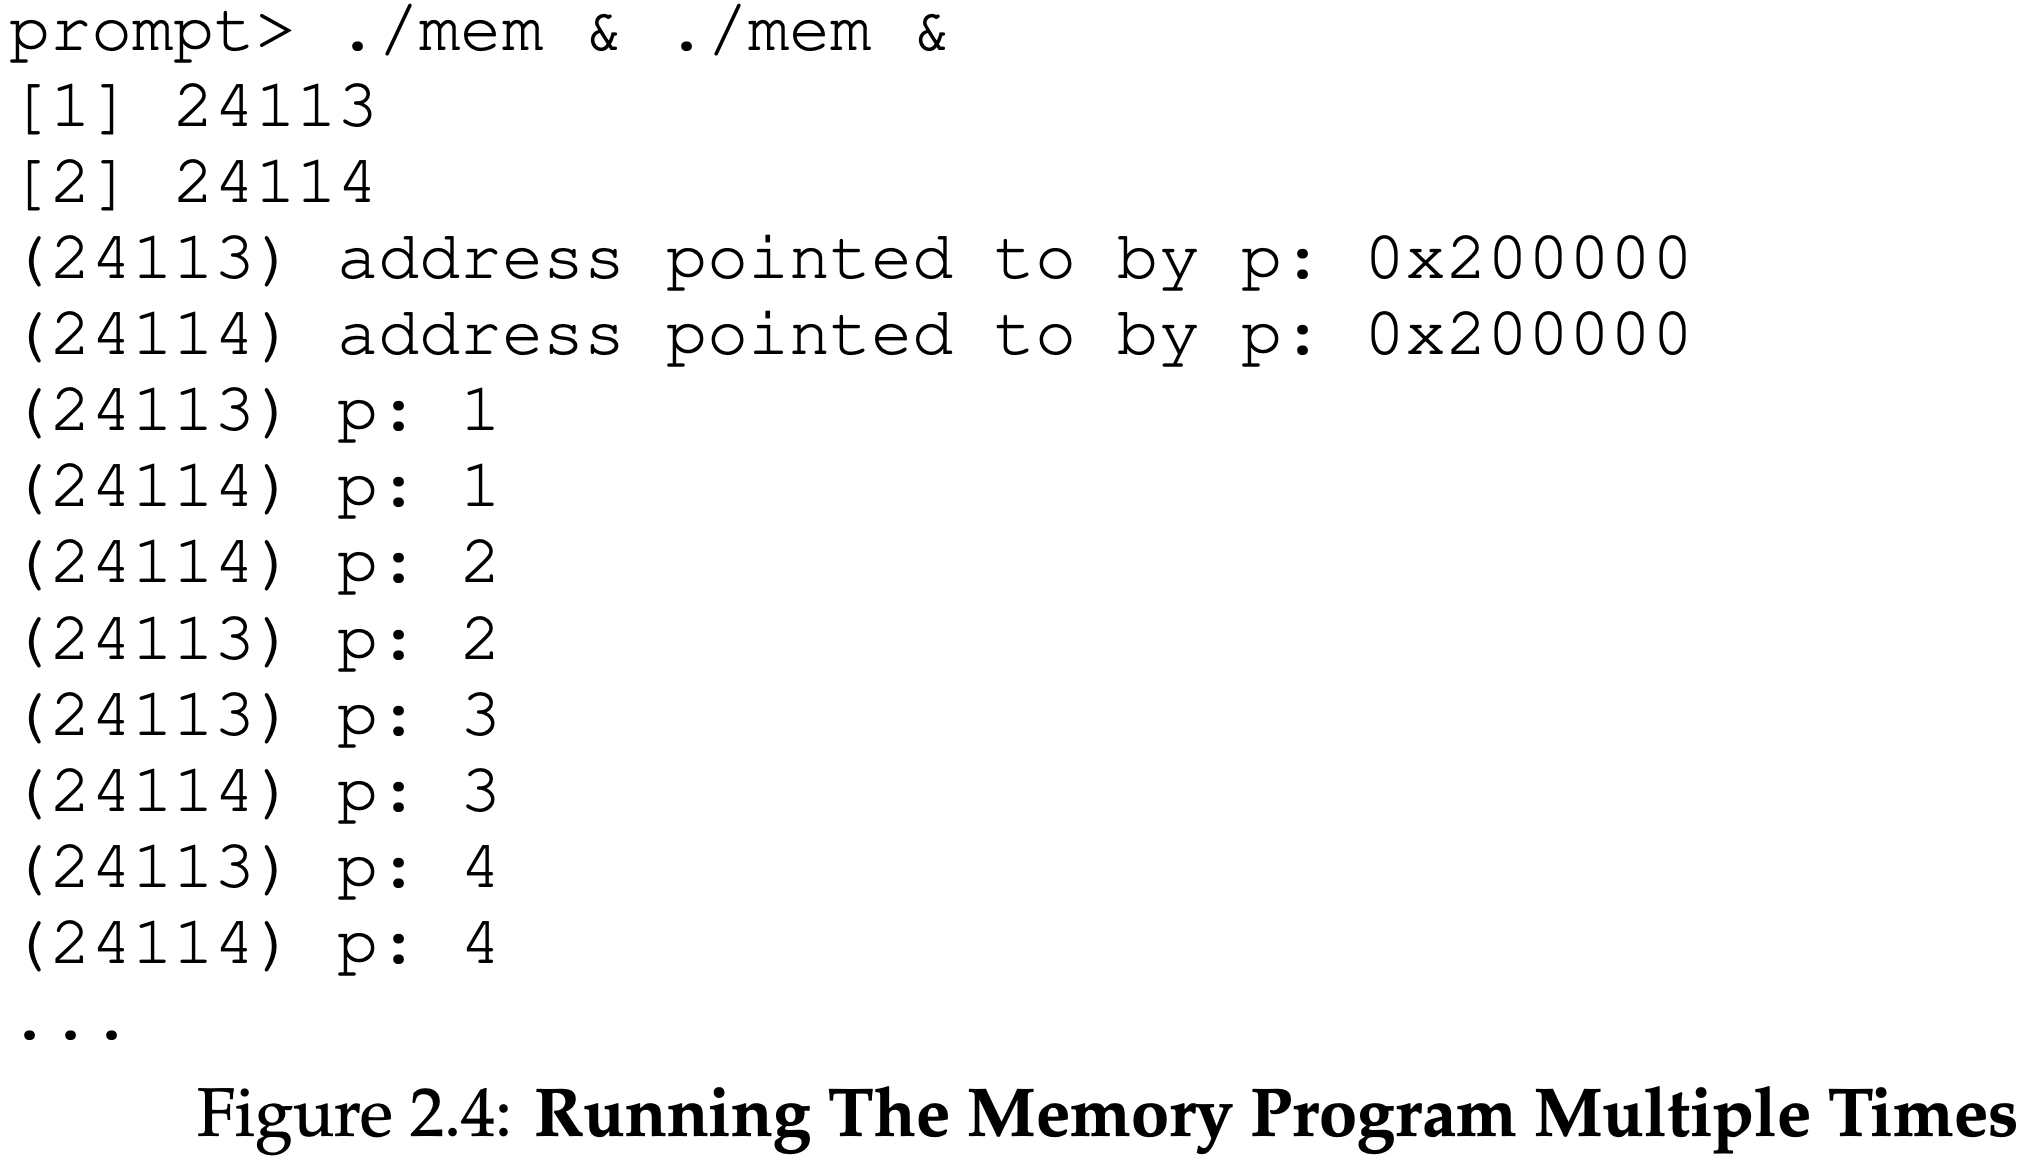
\includegraphics[width=1.1\linewidth]{figs/chapter-2/figure-2.4.png}
        \caption*{Source: chapter page 6.}
        \label{fig:figure-2.4}
    \end{figure}
      % \figureplaceholder{Figure 2.4: Running the Memory Program Multiple Times}{Place the book figure here. Source: chapter page 6.}

    \column{0.50\textwidth}
      \begin{itemize}
        \item Two processes can appear to use the same address independently.
        \item Each process sees its own private \textbf{virtual address space}.
        \item The OS maps each virtual address space onto shared physical memory.
        \item One process normally does not affect another process's address space.
      \end{itemize}
  \end{columns}
\end{frame}

% Slide 7
\begin{frame}{Concurrency}
  \begin{columns}[T,onlytextwidth]
    \column{0.48\textwidth}
      \begin{itemize}
        \item Concurrency refers to problems that arise when multiple activities proceed at the same time.
        \item Modern programs may contain multiple threads sharing the same memory space.
        \item The example creates two worker threads that increment a shared counter.
      \end{itemize}

    \column{0.50\textwidth}
    \begin{figure}
        \centering
        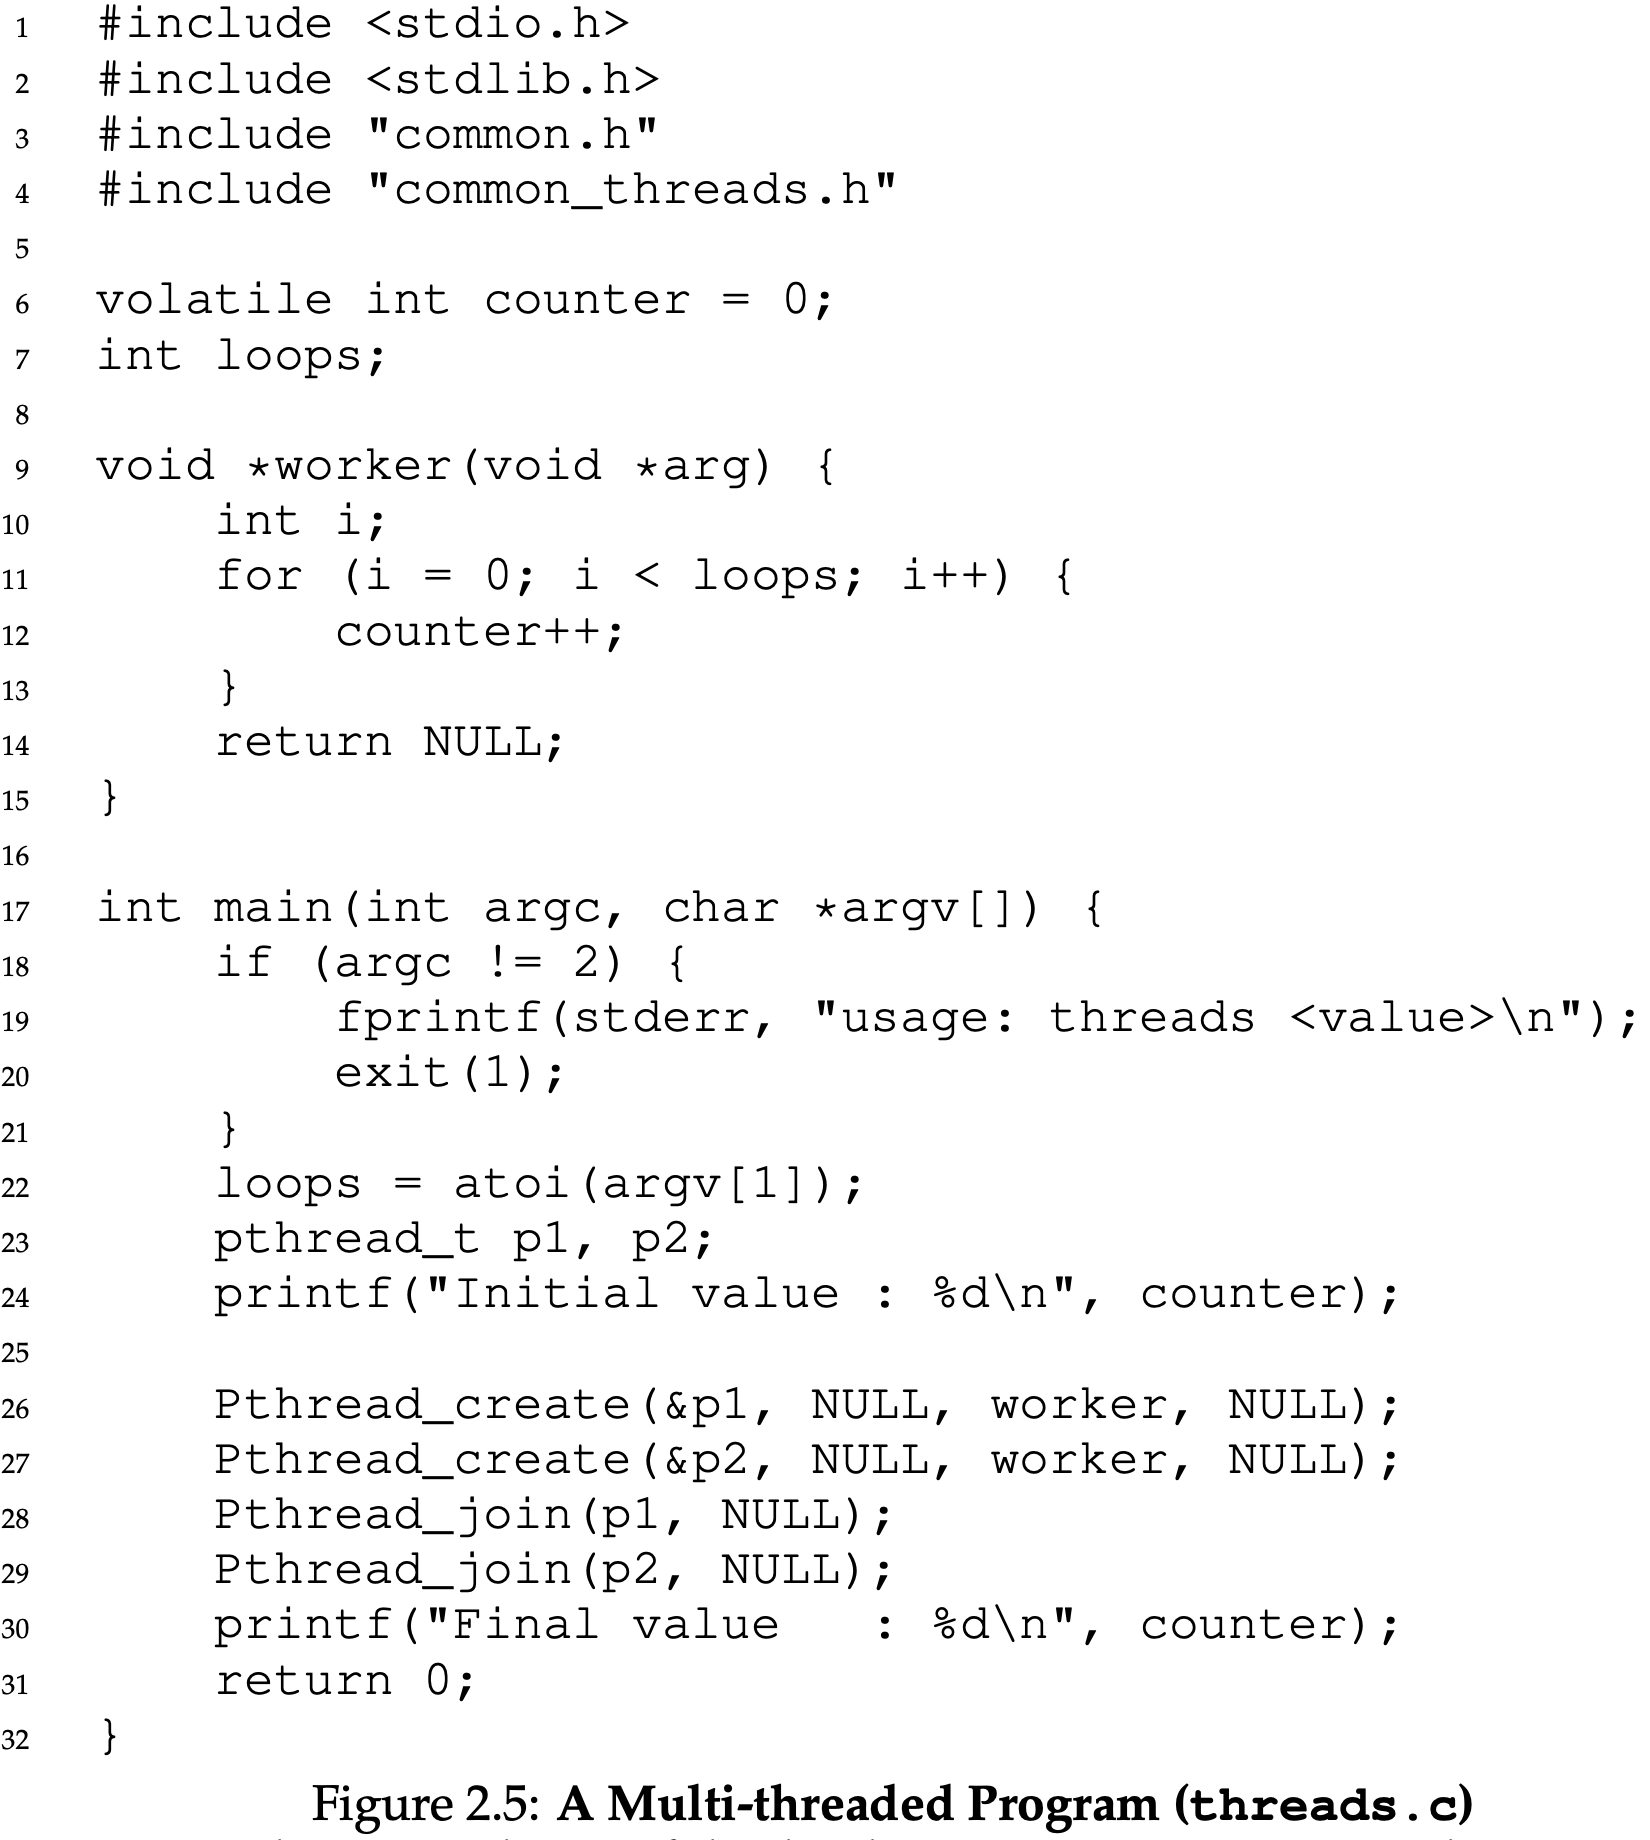
\includegraphics[width=1.1\linewidth]{figs/chapter-2/figure-2.5.png}
        \caption*{Source: chapter page 7.}
        \label{fig:figure-2.5}
    \end{figure}
      % \figureplaceholder{Figure 2.5: threads.c}{Place the book figure here. Source: chapter page 7.}
  \end{columns}
\end{frame}

% Slide 8
\begin{frame}{Why Concurrency Is Difficult}
  \begin{itemize}
    \item With 1,000 increments per thread, the expected final value can be observed.
    \item With larger loop counts, the program may produce incorrect and different results.
    \item Incrementing a shared counter requires multiple machine instructions.
    \item Because the operation is not atomic, thread interleavings can produce unexpected outcomes.
  \end{itemize}

  \vspace{0.5em}
  \begin{alertblock}{The Crux of the Problem}
    How can we build correct programs when many threads execute concurrently in the same memory space?
  \end{alertblock}

  % Source location: shaded ``Crux of the Problem'' box, chapter page 9.
\end{frame}

% Slide 9
\begin{frame}{Persistence}
  \begin{columns}[T,onlytextwidth]
    \column{0.48\textwidth}
      \begin{itemize}
        \item Main memory is volatile: data can disappear after power loss or a crash.
        \item Persistent storage keeps data for the long term.
        \item The file system manages persistent data on storage devices.
        \item Applications use system calls such as \texttt{open()}, \texttt{write()}, and \texttt{close()}.
      \end{itemize}

    \column{0.50\textwidth}
    \begin{figure}
        \centering
        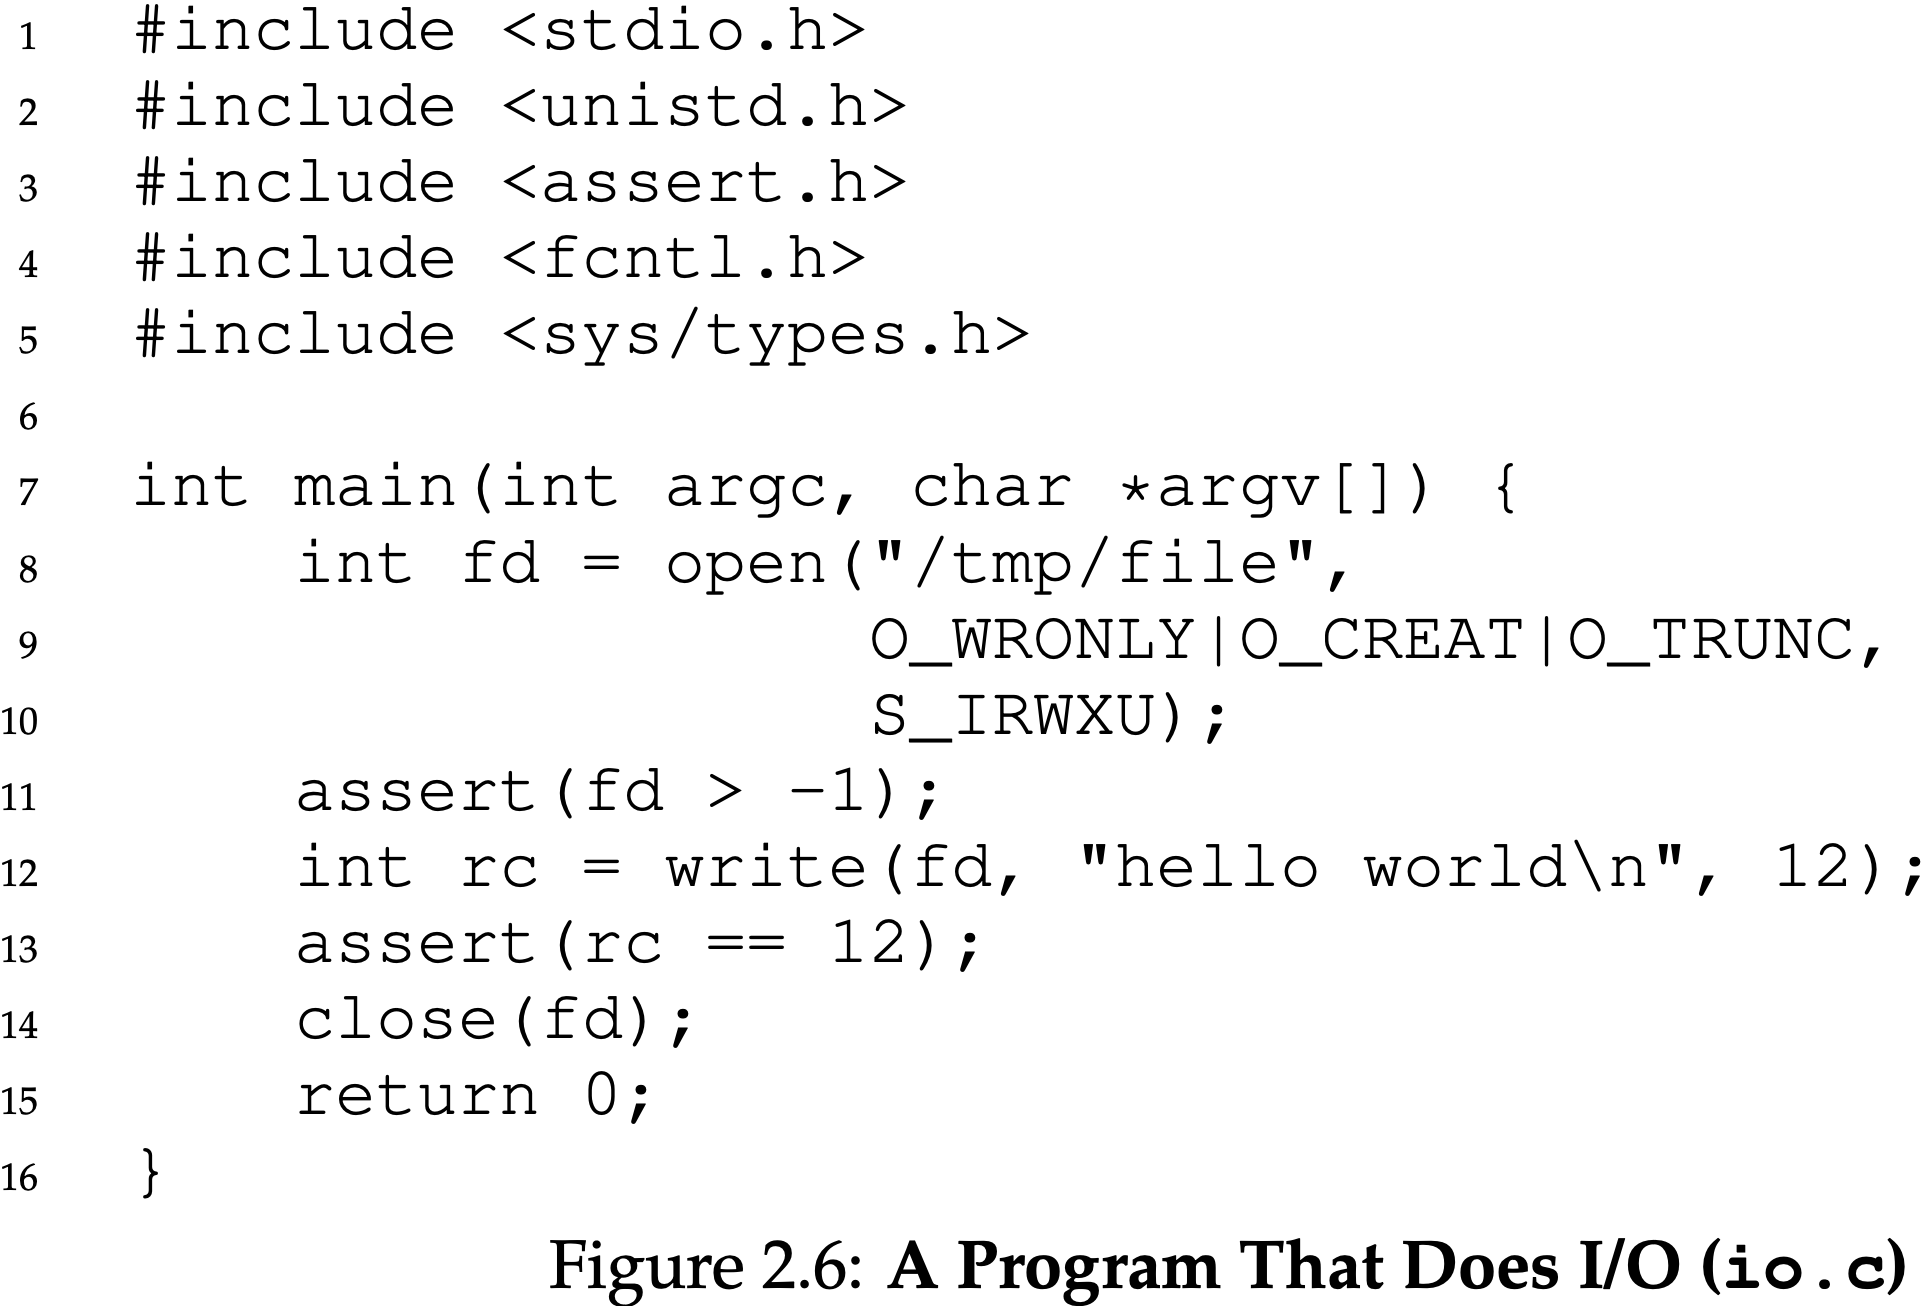
\includegraphics[width=1.1\linewidth]{figs/chapter-2/figure-2.6.png}
        \caption*{Source: chapter page 10.}
        \label{fig:figure-2.6}
    \end{figure}
      % \figureplaceholder{Figure 2.6: io.c}{Place the book figure here. Source: chapter page 10.}
  \end{columns}
\end{frame}

% Slide 10
\begin{frame}{Reliable Persistent Storage}
  \begin{itemize}
    \item File systems must determine where data is stored and maintain metadata about it.
    \item They issue I/O requests to underlying storage devices.
    \item For performance, writes may be delayed and grouped.
    \item Techniques such as \textbf{journaling} and \textbf{copy-on-write} help systems recover from failures.
  \end{itemize}

  \vspace{0.5em}
  \begin{alertblock}{The Crux of the Problem}
    How can the OS store data persistently with correctness, performance, and reliability?
  \end{alertblock}

  % Source location: shaded ``Crux of the Problem'' box, chapter page 11.
\end{frame}

% Slide 11
\begin{frame}{Operating System Design Goals}
  \begin{itemize}
    \item \textbf{Abstraction:} make the system convenient and manageable.
    \item \textbf{Performance:} minimize time and space overheads.
    \item \textbf{Protection and isolation:} prevent applications from harming one another or the OS.
    \item \textbf{Reliability:} keep the operating system running correctly.
    \item Additional goals may include energy efficiency, security, and mobility.
  \end{itemize}
\end{frame}

% Slide 12
\begin{frame}{A Brief History of Operating Systems}
  \begin{enumerate}
    \item \textbf{Early systems:} OS as libraries of common functions; batch processing.
    \item \textbf{Protection:} system calls, user mode, kernel mode, and controlled privilege transitions.
    \item \textbf{Multiprogramming:} several jobs in memory, rapid switching, better CPU utilization.
    \item \textbf{UNIX:} simple, powerful abstractions and tools; strong influence on later systems.
    \item \textbf{Modern era:} mature OS ideas returned to personal computers and later to mobile systems.
  \end{enumerate}

  % Optional visual reference from the chapter:
  % - ``The Importance of UNIX'' aside: chapter page 15.
  % - ``And Then Came Linux'' aside: chapter page 16.
\end{frame}

% Slide 13
\begin{frame}{Chapter Summary}
  \begin{block}{Three Major Themes}
    \begin{enumerate}
      \item \textbf{Virtualization} of the CPU and memory.
      \item \textbf{Concurrency} and correct coordination among simultaneous activities.
      \item \textbf{Persistence} through devices and file systems.
    \end{enumerate}
  \end{block}

  \vspace{0.5em}
  \begin{itemize}
    \item The OS provides abstractions and interfaces that make hardware easier to use.
    \item It manages resources while pursuing performance, protection, and reliability.
  \end{itemize}
\end{frame}

% ---------------------------------------------------------
\begin{frame}{Part I --- Virtualization}

\begin{center}
    \Huge
    \textbf{Virtualization}
\end{center}

\end{frame}
